\documentclass[submit]{../harvardml}

\course{CS1810-S25}
\assignment{Homework \#2}
\duedate{February 28, 2025 at 11:59 PM}

\usepackage{../common}
\usepackage[OT1]{fontenc}
\usepackage[colorlinks,citecolor=blue,urlcolor=blue]{hyperref}
\usepackage{graphicx}
\usepackage{subfig}
\usepackage{fullpage}
\usepackage{amsmath}
\usepackage{amssymb}
\usepackage{framed}
\usepackage{color}
\usepackage{soul}
\usepackage{todonotes}
\usepackage{listings}
\usepackage{enumitem}
\usepackage{bm}
\usepackage{bbm}
\usepackage{float}
\usepackage{mathtools}
\usepackage{xcolor} % For table colors
\usepackage{booktabs} % For better table formatting
\usepackage{colortbl}
\usepackage{makecell} % For multi-line cells

\newcommand{\B}{\text{B}}
\newcommand{\Beta}{\text{Beta}}

\usepackage[mmddyyyy,hhmmss]{datetime}

\definecolor{verbgray}{gray}{0.9}

\lstnewenvironment{csv}{%
  \lstset{backgroundcolor=\color{verbgray},
  frame=single,
  framerule=0pt,
  basicstyle=\ttfamily,
  columns=fullflexible}}{}
  

%%%%%%%%%%%%%%%%%%%%%%%%%%%%%%%%%%
%% Solution environment
\usepackage{xcolor}
\usepackage{comment}
\newenvironment{solution}
  {\color{blue}\section*{Solution}}
{}
%%%%%%%%%%%%%%%%%%%%%%%%%%%%%%%%%%

\begin{document}

\begin{center}
  {\Large Classification and Bias-Variance Trade-offs}\\
\end{center}

\subsection*{Introduction}

This homework is about classification, bias-variance trade-offs, and
uncertainty quantification.

The datasets that we will be working with relate to astronomical observations and loan applicants
The first dataset, found at \verb|data/planet-obs.csv|,
contains information on whether a planet was observed (as a binary
variable) at given points in time. This will be used in Problem 1. The
second dataset, available at \verb|data/hr.csv|, details different
loan applicants and their measured debt to income ratio and credit score. You will
work with this data in Problem 3.

As a general note, for classification problems we imagine that we have
the input matrix $\boldX \in \reals^{n \times d}$ (or perhaps they
have been mapped to some basis $\bm{\Phi}$, without loss of
generality) with outputs now ``one-hot encoded."  This means that if
there are~$K$ output classes, rather than representing the output
label $y$ as an integer~${1,2,\ldots,K}$, we represent $\boldy$ as a
``one-hot" vector of length~$K$. A ``one-hot" vector is defined as
having every component equal to 0 except for a single component which
has value equal to 1.  For example, if there are $K = 7$ classes and a
particular data point belongs to class 3, then the target vector for
this data point would be~$\boldy = [0,0,1,0,0,0,0]$.  We will define
$C_1$ to be the one-hot vector for the 1st class, $C_2$ for the 2nd
class, etc.  Thus, in the previous example $\boldy = C_3$. If there
are $K$ total classes, then the set of possible labels is $\{C_1
  \ldots C_K \} = \{C_k\}_{k=1}^K$.  Throughout the assignment we will
assume that each label $\boldy \in \{C_k\}_{k=1}^K$ unless otherwise
specified. The most common exception is the case of binary
classification ($K = 2$), in which case labels are the typical
integers $y \in \{0, 1\}$.

\subsection*{Resources and Submission Instructions}

We encourage you to read CS181 Textbook's Chapter 3 for more
information on linear classification, gradient descent, and
classification in the discriminative setting. Read Chapter 2.8 for
more information on the trade-offs between bias and variance.

In problems 1 and 3, you may use \texttt{numpy} or \texttt{scipy}, but
not \texttt{scipy.optimize} or \texttt{sklearn}. Example code is given
in the provided notebook. \textbf{We highly recommend that you use Google Colab for problems 1 and 3 to avoid numerical stability issues.}

Please type your solutions after the corresponding problems using this
\LaTeX\ template, and start each problem on a new page.

Please submit the \textbf{writeup PDF to the Gradescope assignment
  `HW2'}. Remember to assign pages for each question.  Please submit
your \textbf{\LaTeX\ file and code files to the Gradescope assignment
  `HW2 - Supplemental'}. \textbf{You must include your plots in your
  writeup PDF. } The supplemental files will only be checked in
special cases, e.g. honor code issues, etc.


%%%%%%%%%%%%%%%%%%%%%%%%%%%%%%%%%%%%%%%%%%%%%
% Problem 1
%%%%%%%%%%%%%%%%%%%%%%%%%%%%%%%%%%%%%%%%%%%%%

\begin{problem}[Exploring Bias-Variance and Uncertainty]
In this problem, we will explore the bias and variance of a few
different model classes when it comes to logistic regression and
investigate two sources of predictive uncertainty in a synthetic
(made-up) scenario.

We are using a powerful telescope in the northern hemisphere to gather
measurements of some planet of interest. At certain times however, our
telescope is unable to detect the planet due to its positioning around
its star.  The data in \verb|data/planet-obs.csv| records the
observation time in the ``Time" column and whether the planet was
detected in the ``Observed" column (with the value 1 representing that
it was observed).  These observations were taken over a dark, clear
week, which is representative of the region.  Since telescope time is
expensive, we would like to build a model to help us schedule and find
times when we are likely to detect the planet.

\begin{enumerate}
  \item Split the data into 10 mini-datasets of size $N = 30$ (i.e. dataset 1 consists of the first 30 observations, dataset 2 consists of the next 30, etc. This has already been done for you). Consider the three bases $\boldsymbol\phi_1(t) = [1, t]$, $\boldsymbol\phi_2(t) = [1,
          t, t^2]$, and $\boldsymbol\phi_3(t) = [1, t, t^2, t^3, t^4, t^5]$. For each of these bases, fit a logistic regression model using sigmoid($\boldw^\top \boldsymbol\phi(t)$) to each dataset by using gradient descent to
        minimize the negative log-likelihood.  This means you will be
        running gradient descent 10 times for each basis, once for each
        dataset.

        Use the given starting values of $\boldw$ and a learning rate of $\eta=0.001$, take 1,000 update
        steps for each gradient descent run, and make sure to average the
        gradient over the data points at each step. These parameters,
        while not perfect, will ensure your code runs reasonably quickly.

  \item After consulting with a domain expert, we find that the probability of observing the planet is periodic as the planet revolves around its star---we are more likely to observe the planet when it is in front of its star than when it is behind it. In fact, the expert determines that observation follows the generating process $y \sim \text{Bern}(f(t))$, where $f(t) = 0.4 \times \cos(1.1t + 1) + 0.5$ for $t \in [0, 6]$ and $y \in \{0,1\}$. Note that we, the modelers, do not usually see the true data distribution. Knowledge of the true $f(t)$ is only exposed in this problem to allow for verification of the true bias.

        Use the given code to plot the true process versus your learned models. Include your plots in your solution PDF.

        \textbf{In no more than 5 sentences}, explain how bias and variance reflected in the 3 types of curves on the graphs.  How do the fits of the individual and mean prediction functions change?  Keeping in mind that none of the model classes match the true generating process exactly, discuss the extent to which each of the bases approximates the true process.

\end{enumerate}
\end{problem}

\newpage
\begin{framed}
  \noindent\textbf{Problem 1} (cont.)\\
  \begin{enumerate}
    \setcounter{enumi}{2}

    \item If we were to increase the size of each dataset drawn from $N = 30$ to a larger number, how would the bias and variance change for each basis? Why might this be the case? You may experiment with generating your own data that follows the true process and plotting the results, but this is \textbf{not} necessary. \textbf{Your response should not be longer than 5 sentences}.

    \item Consider the test point $t = 0.1$. Using your models trained on basis $\boldsymbol\phi_3$, report the predicted probability of observation of the \textit{first} model (the model trained on the first 30 data points). How can we interpret this probability as a measure of uncertainty? Then, compute the variance of the classification probability over your 10 models at the same point $t = 0.1$. How does this measurement capture another source of uncertainty, and how does this differ from the uncertainty represented by the classification probability? Repeat this process (reporting the first model's classification probability and the variance over the 10 models) for the point $t = 3.2$.

          Compare the uncertainties and their sources at times $t=0.1$ and $t=3.2$.

    \item We now need to make some decisions about when to request time on
          the telescope.  The justifications of your decisions will be sent to
          your funding agency, which will determine whether you will be
          allocated funds to use the telescope for your project. \textbf{In no more than 10 lines}, answer the following questions.
          \begin{itemize}
            \item To identify the ideal time, which model(s) would you use and why?
            \item What time would you request, and why?
            \item Your funding agency suggests using a different telescope in a
                  humid area near the equator. Can you still use your model to
                  determine when the planet is likely to be visible?  Why? Are there
                  adaptations that may be necessary?
            \item You seek out a team that has used the alternative telescope
                  for observing this planet, and they provide you their observation
                  file \verb|data/planet-obs-alternate.csv|.
                  Compare the observations from your telescope to theirs.  What
                  seems to be happening?  What might be an appropriate model for
                  this? Your funding agency asks you to refit your models on these
                  new data.  Do you think this is a reasonable ask, and if so, how
                  will it help you make better decisions about when to request
                  viewing time?  If not, why do you think the additional modeling
                  will not help? You do \emph{not} need to do any modeling for this
                  question!

          \end{itemize}
          In these questions, we are looking for your reasoning; there may be
          more than one valid answer.

  \end{enumerate}
\end{framed}

\newpage

\begin{solution}

\begin{enumerate}
    \item [1.] See \texttt{hw2.ipynb}.
    \item [2.] The plots are included in Figures 1.2.1-3 below.
    \begin{figure}[H]
        \centering
        \includegraphics[width=0.65\textwidth]{img_output/basis1.png}
        \caption*{\textcolor{blue}{Figure 1.2.1: Models for basis 1}}
        \label{fig:q1.2a}
    \end{figure}
    \begin{figure}[H]
        \centering
        \includegraphics[width=0.65\textwidth]{img_output/basis2.png}
        \caption*{\textcolor{blue}{Figure 1.2.2: Models for basis 2}}
        \label{fig:q1.2b}
    \end{figure}
    \begin{figure}[H]
        \centering
        \includegraphics[width=0.65\textwidth]{img_output/basis3.png}
        \caption*{\textcolor{blue}{Figure 1.2.3: Models for basis 3}}
        \label{fig:q1.2c}
    \end{figure}
    Bias measures how much predictions deviate from the truth, while variance reflects sensitivity to changes in the training set, seen in how much the individual 10 models differ from one another. The bias-variance tradeoff, which means reducing bias increases variance and vice versa. Basis 1 has high bias (black line deviates from green) but low variance (individual models are similar). Basis 2 lowers bias (black line follows green better) but increases variance (greater spread among models). Basis 3 further reduces bias (but not my a lot) but has much higher variance, evident in the large deviations between individual models, leading to overfitting. Thus, the model under basis 2 approximates the true generating process best, as it balances bias against variance, ensuring that it fits the train data moderately well, whilst also generalizing.

    \vspace{.5em}
    (Note that the purple curves are strictly worse than the black curves because each purple curve is based on a single dataset, while the black curve represents the average of 10 different purple curves. As a result, the purple curves suffer from both the bias inherent to the chosen basis (deviating from the ground truth) and significantly higher variance compared to the mean prediction. This is why we excluded the purple curves from our main discussion.)

    \item [3.] Assuming that the number of datasets stays at 10, then increasing the size of each dataset from $N=30$ to a larger number will decrease variance, though the effect on bias is less clear. For larger $N$, estimates of the model parameters should become more stable as each dataset now likely captures more of the underlying pattern. The individual models will therefore be more consistent with one another, reducing the spread between them as identified in part (2). By contrast, the bias may still remain. For example, the model under basis 1 is too simple and systematically underfits the data (does not capture the curvature enough). Thus, having more data points will improve and reduce the variance in our parameter estimates... but these parameters are in the fundamentally wrong model! 

\clearpage
    \item [4.] Table 1.4.1 details the predicted probabilities and variances:
\begin{table}[H]
    \centering
    \renewcommand{\arraystretch}{1.3} % Adjust row height
    \arrayrulecolor{blue} % Set border color to blue
    \begin{tabular}{|c|c|c|}
        \hline
        \textcolor{blue}{\textbf{Time / Metric}} & \textcolor{blue}{\makecell{\textbf{Predicted prob. of obs.} \\ \textbf{based on 1st model}}} & \textcolor{blue}{\textbf{Variance over 10 models}} \\
        \hline
        \textcolor{blue}{$\pmb{t = 0.1}$} & \textcolor{blue}{0.8110} & \textcolor{blue}{0.1060} \\
        \hline
        \textcolor{blue}{$\pmb{t = 3.2}$} & \textcolor{blue}{1.0} & \textcolor{blue}{0.24} \\
        \hline
    \end{tabular}
    \caption*{\textcolor{blue}{Table 1.4.1: Classification Probabilities and Model Variances}}
    \label{tab:classification_variances}
\end{table}
    We can interpret the predicted probability of observation of the first model as how ``certain'' we are that the planet will be detectable at time $t=0.1$. So we are around 81\% certain that we will be able to detect the planet at $t=0.1$, with $100\% - 81\% = 19\%$ representing our uncertainty. By similar reasoning, we are apparently 100\% certain that we will be able to detect the planet at $t=3.2$. This should raise some skepticism, as how can we be 100\% sure we will be able to observe the planet at exactly $t=3.2$?

    \vspace{.5em}
    This is where the variance comes into play, which captures the uncertainty in our prediction. Higher variance corresponds to greater uncertainty. Indeed, we can see that we are much less certain our prediction for $t=3.2$ than $t=0.1$, capturing our skepticism of the predicted 100\%.
    
    \vspace{.5em}
    To summarize, there are two distinct layers of uncertainty at play:
    \begin{enumerate}
        \item [1.] Uncertainty in whether the planet is detectable at a given $t$ (captured by the predicted probability).
        \item [2.] Uncertainty in our confidence about this detection probability (captured by the variance of the prediction).
    \end{enumerate}

    \item [5.] We seek an accurate model that generalizes well beyond the training set. As discussed in part (2), the mean model under basis 2 achieves this best, so we select it as our model.

    \vspace{.5em}
We want a time $t$ where the predicted observation probability is high and variance is low, so that we have confidence in our detection. From Figure 1.2.2, $t=6$ is ideal, but since it is outside our training range, we opt for $t \approx 5.6$. While the true maximum is at $t \approx 4.8$, we lack access to the ground truth model.

    \vspace{.5em}
    If the area is humid, visibility may worsen, and we must assess the new telescope’s quality relative to our original. Latitude differences could also affect detectability (e.g., the planet may not be geometrically visible from the equator, in which case we know that there is probability zero of us detecting it, at any time $t$). If we account for these factors, the model may still provide predictions, but with higher variance.

    \vspace{.5em}
    Plotting both telescopes’ observations suggests they sometimes detect the planet at different times, likely due to instrumental or environmental factors. A better model would incorporate extra predictors for these influences. Refitting with this expanded dataset could improve generalization (in particular for environmental/instrumental factors), reducing the variance in our predictions.
\end{enumerate}
\end{solution}

%%%%%%%%%%%%%%%%%%%%%%%%%%%%%%%%%%%%%%%%%%%%%
% Problem 2
%%%%%%%%%%%%%%%%%%%%%%%%%%%%%%%%%%%%%%%%%%%%%

\begin{problem}[Maximum likelihood in classification]

Consider now a generative $K$-class model.  We adopt class prior
$p(\boldy = C_k; \bpi) = \pi_k$ for all $k \in \{1, \ldots, K\}$
(where $\pi_k$ is a parameter of the prior).
Let  $p(\boldx|\boldy=C_k)$ denote
the class-conditional density of features $\boldx$ (in this
case for class $C_k$). Consider the data set $D = \{(\boldx_i,
  \boldy_i)\}_{i=1}^n$ where as above $\boldy_i \in \{C_k\}_{k=1}^K$ is
encoded as a one-hot target vector and the data are independent.

\begin{enumerate}
  \item Write out the log-likelihood of the data set, $\ln p(D ; \bpi)$.

  \item Since the prior forms a distribution, it has the constraint that
        $\sum_k\pi_k - 1 = 0$.  Using the hint on
        Lagrange multipliers below, give the
        expression for the maximum-likelihood estimator for the prior
        class-membership probabilities, i.e.
        $\hat \pi_k.$
        Make sure to write out the intermediary equation you need
        to solve to obtain this estimator. Briefly state why your final answer is intuitive.
\end{enumerate}

For the remaining questions, let the
class-conditional probabilities be Gaussian distributions with
the same covariance matrix
$$p(\boldx | \boldy = C_k) = \mathcal{N}(\boldx |  \bmu_k, \bSigma), \text{\ for\ }k \in \{1,\ldots, K\}$$
and different means $\bmu_k$ for each class.

\begin{enumerate}
  \item[3.] Derive the gradient of the log-likelihood with respect to vector $\bmu_k$.
    Write the expression in matrix form as a function of the variables defined
    throughout this exercise. Simplify as much as possible for full credit.
  \item[4.] Derive the maximum-likelihood estimator $\hat{\mu}_k$ for vector $\bmu_k$. Briefly state why your final answer is intuitive.
  \item[5.] Derive the gradient for the log-likelihood with respect to the
    covariance matrix $\bSigma$ (i.e., looking
    to find an MLE for the covariance).
    Since you are differentiating with respect to a
    \emph{matrix}, the resulting expression should be a matrix!
    %
  \item[6.] Derive the maximum likelihood estimator $\hat{\Sigma}$ of the covariance matrix.
\end{enumerate}

\paragraph{Hint: Lagrange Multipliers.} Lagrange Multipliers are a method for
optimizing a function $f$ with respect to an
equality constraint, i.e.
\[\min_{\boldx} f(\boldx)\ \text{s.t.}\ g(\boldx) = 0.\]

This can be turned into an unconstrained problem by introducing a
Lagrange multiplier $\lambda$ and constructing the Lagrangian function,
\[L(\boldx, \lambda) =  f(\boldx) + \lambda g(\boldx).\]

It can be shown that it is a necessary condition that the optimum
is a critical point of this new function. We can find this point by solving two equations:

\[\frac{\partial L(\boldx, \lambda)}{\partial  \boldx} = 0  \ \ \text{and}\  \  \frac{\partial L(\boldx, \lambda)}{\partial \lambda} = 0 \]


\paragraph{Cookbook formulas.} Here are some formulas you might want to consider
using to compute difficult gradients. You can use them  in the homework
without proof. If you are looking to hone your matrix calculus skills, try to
find different ways to prove these formulas yourself (will not be part of the
evaluation of this homework). In general, you can use any formula from the matrix cookbook,
as long as you cite it. We opt for the following common notation:
$\boldX^{-\top} := (\boldX^{\top})^{-1}$
\begin{align*}
   & \frac{\partial \bolda^\top \boldX^{-1} \boldb}{\partial \boldX} = - \boldX^{-\top} \bolda \boldb^\top \boldX^{-\top} \\
   & \frac{\partial \ln | \det (\boldX) |}{\partial \boldX} = \boldX^{-\top}
\end{align*}
\end{problem}

\newpage

\begin{solution}

\begin{enumerate}
    \item [1.] Since the data are independent,
    \begin{align*}
        p(D; \bpi) &= p\left( \left\{ (\boldx_i, \boldy_i) \right\}_{i=1}^n ; \bpi \right) \\
        &= \prod_{i=1}^n p\left( (\boldx_i,\boldy_i) ; \bpi \right) \\
        \therefore \quad \ln p(D; \bpi) &= \sum_{i=1}^n \ln p\left( (\boldx_i,\boldy_i) ; \bpi \right)
        \tag*{(2.1.1)}
    \end{align*}
    Let $y_{ik}$ denote the $k$\textsuperscript{th} entry in the one-hot vector $\boldy_i$. (In other words, $y_{ik}$ is the indicator that data point $i$ belongs to class $k$.) Then
    \begin{align*}
        p(\boldx_i, \boldy_i; \bpi) &= \prod_{k=1}^K p(\boldx_i, \boldy_i = C_k; \bpi)^{y_{ik}} \\
        \therefore \quad \ln p(\boldx_i, \boldy_i; \bpi) &= \sum_{k=1}^K y_{ik} \ln p(\boldx_i, \boldy_i = C_k; \bpi) \tag*{(2.1.2)}
    \end{align*}
    Combining (2.1.2) with (2.1.1) gives
    \begin{align*}
        \ln p(D; \bpi) &= \sum_{i=1}^n \sum_{k=1}^K y_{ik} \ln p(\boldx_i, \boldy_i = C_k; \bpi) \tag*{(2.1.3)}
    \end{align*}
    Now, note that
    \begin{align*}
        p(\boldx_i, \boldy_i=C_k; \bpi) &= p(\boldx_i | \boldy_i = C_k)\Pr(\boldy_i = C_k; \bpi) \\
        &= p(\boldx_i | \boldy_i = C_k) \cdot \pi_k \tag*{(2.1.4)}
    \end{align*}
    Combining (2.1.4) with (2.1.3) gives
    \begin{align*}
        \Aboxed{ \ln p(D; \bpi) &= \sum_{i=1}^n \sum_{k=1}^K y_{ik} \left\{ \ln p(\boldx_i | \boldy_i = C_k) + \ln \pi_k \right\} } \tag*{(2.1.4)}
    \end{align*}

    \item[2.] Let $f(\bpi) = \ln p(D; \bpi)$ and $g(\bpi) = \sum_{k=1}^K \pi_k - 1$. We seek to maximize $f$ subject to the constraint $g=0$. We do so by constructing the Lagrangian
    \begin{align*}
        L(\bpi, \lambda) &= f(\bpi) + \lambda g(\bpi) \tag*{(2.2.1)}
    \end{align*}
    where $\lambda$ denotes the Lagrangian multiplier.

    \vspace{.5em}
    Computing the gradient yields
    \begin{align*}
        \nabla_{\bpi} L(\bpi, \lambda) &= \left( \frac{\partial L}{\partial \pi_1}, \frac{\partial L}{\partial \pi_2}, \ldots, \frac{\partial L}{\partial \pi_K} \right) \\
        &= \left( \frac{1}{\pi_1}\sum_{i=1}^ny_{i1}, \frac{1}{\pi_2}\sum_{i=1}^ny_{i2}, \ldots, \frac{1}{\pi_K}\sum_{i=1}^ny_{iK} \right) + \lambda(1,1,\ldots,1) \tag*{(2.2.2)}
    \end{align*}
    noting that $\ln p(\boldx_i | \boldy_i = C_k)$ is independent of $\bpi$.

    \clearpage
    To find all critical points, we set the expression in (2.2.2) to 0, which gives
    \begin{align*}
        -\lambda = \frac{1}{\pi_1}\sum_{i=1}^ny_{i1} = \frac{1}{\pi_2}\sum_{i=1}^ny_{i2} = \ldots = \frac{1}{\pi_K}\sum_{i=1}^ny_{iK} \tag*{(2.2.3)}
    \end{align*}
    and hence
    \begin{align*}
        \pi_k = -\frac{1}{\lambda} \sum_{i=1}^n y_{ik} \tag*{(2.2.4)}
    \end{align*}
    for $k = 1,2,\ldots,K$.

    \vspace{.5em}
    Recall the constraint
    \begin{align*}
        g(\bpi) = \sum_{k=1}^K \pi_k - 1 = 0 \tag*{(2.2.5)}
    \end{align*}
    Combining this with (2.2.4) gives
    \begin{align*}
        -\frac{1}{\lambda} \sum_{k=1}^K \sum_{i=1}^n y_{ik} - 1 &= 0 \\
        \therefore \quad \lambda = -\sum_{i=1}^n \sum_{k=1}^K y_{ik} = -\sum_{i=1}^n 1 = -n \tag*{(2.2.6)}
    \end{align*}
    since each data point must belong to exactly one class.

    \vspace{.5em}
    Combining this with (2.2.4) gives us the MLE
    \begin{align*}
        \Aboxed{ \hat{\pi}_k &= \frac{1}{n}\sum_{i=1}^n y_{ik} } \tag*{(2.2.7)}
    \end{align*}
    \textbf{Intuition:} The MLE for $\pi_k$---the \textit{unconditional} probability that one of our data points falls into class $k$---is the \textit{proportion} of data points that fall into class $k$. 

    \item[3.] We have that
    \begin{align*}
        p(\boldx_i | \boldy_i = C_k) &= \mathcal{N}(\boldx_i | \bmu_k, \bSigma) \\
        &= \frac{1}{(2\pi)^{n/2}|\bSigma|^{1/2}}\exp \left\{ -\frac{1}{2}(\boldx_i - \bmu_k)^{\mathrm{T}} \bSigma^{-1} (\boldx_i - \bmu_k) \right\} \\
        \therefore \quad \ln p(\boldx_i | \boldy_i = C_k) &= -\frac{n}{2}\ln 2\pi - \frac{1}{2} \ln |\bSigma| - \frac{1}{2} (\boldx_i - \bmu_k)^{\mathrm{T}} |\bSigma|^{-1} (\boldx_i - \bmu_k) \tag*{(2.3.1)}
    \end{align*}
    Combining this with the expression for log-likelihood in (2.1.4),
    \begin{align*}
        \frac{\partial \ln p(D; \bpi)}{\partial \bmu_k} &= \sum_{i=1}^n \sum_{k=1}^K y_{ik}\left(-\frac{1}{2}\right)2\left(\bSigma^{-1}\right)(\boldx_i - \bmu_k)(-1) \\
        \therefore \quad \Aboxed{ \frac{\partial \ln p(D; \bpi)}{\partial \bmu_k} &= \left(\bSigma^{-1}\right)\sum_{i=1}^n y_{ik} (\boldx_i - \bmu_k) } \tag*{(2.3.2)}
    \end{align*}
    \item[4.] Setting the expression in (2.3.2) to 0 gives
    \begin{align*}
        \sum_{i=1}^n y_{ik}(\boldx_i - \bmu_k) &= 0 \\
        \therefore \quad \Aboxed{ \hat{\bmu}_k = \frac{\sum_{i=1}^n y_{ik}\boldx_i}{\sum_{i=1}^n y_{ik}} } \tag*{(2.4.1)}
    \end{align*}
    \textbf{Intuition:} The MLE for $\bmu_k$ is the average of $\boldx_i$ when considering \textit{only those data points in class $k$}.

    \item[5.] From (2.3.1) and (2.1.4), we have
    \begin{align*}
        \frac{\partial \ln p(D; \bpi)}{\partial \bSigma} &= \sum_{i=1}^n \sum_{k=1}^K y_{ik} \left\{ -\frac{1}{2}\left(\bSigma^{-\mathrm{T}}\right) + \frac{1}{2}\left(\bSigma^{-\mathrm{T}}\right) (\boldx_i - \bmu_k)(\boldx_i - \bmu_k)^\mathrm{T}\left(\bSigma^{-T}\right) \right\} \\
        \therefore \quad \Aboxed{ \frac{\partial \ln p(D; \bpi)}{\partial \bSigma} &= -\frac{n}{2}\left(\bSigma^{-\mathrm{T}}\right) + \frac{1}{2}\left(\bSigma^{-\mathrm{T}}\right)\left\{ \sum_{i=1}^n\sum_{k=1}^K y_{ik} (\boldx_i - \bmu_k)(\boldx_i - \bmu_k)^\mathrm{T} \right\}\left(\bSigma^{-\mathrm{T}}\right) } \tag*{(2.5.1)}
    \end{align*}

    \item[6.] Setting the expression in (2.5.1) to 0 gives
    \begin{align*}
        -\frac{n}{2}\left(\bSigma^{-\mathrm{T}}\right) + \frac{1}{2}\left(\bSigma^{-\mathrm{T}}\right)\left\{ \sum_{i=1}^n\sum_{k=1}^K y_{ik} (\boldx_i - \bmu_k)(\boldx_i - \bmu_k)^\mathrm{T} \right\}\left(\bSigma^{-\mathrm{T}}\right) &= 0
    \end{align*}
    Multiplying by $\left(\bSigma^{-\mathrm{T}}\right)$ on both the left and right gives
    \begin{align*}
        -\frac{n}{2}\bSigma^{\mathrm{T}} + \frac{1}{2}\sum_{i=1}^n\sum_{k=1}^K y_{ik} (\boldx_i - \bmu_k)(\boldx_i - \bmu_k)^\mathrm{T} &= 0 \\
        \therefore \quad \hat{\bSigma}^{\mathrm{T}} &= \frac{1}{n}\sum_{i=1}^n\sum_{k=1}^K y_{ik} (\boldx_i - \bmu_k)(\boldx_i - \bmu_k)^\mathrm{T} \\
        \therefore \quad \Aboxed{ \hat{\bSigma} &= \frac{1}{n}\sum_{i=1}^n\sum_{k=1}^K y_{ik} (\boldx_i - \bmu_k)(\boldx_i - \bmu_k)^\mathrm{T} } \tag*{(2.6.1)}
    \end{align*}
\end{enumerate}

\end{solution}

%%%%%%%%%%%%%%%%%%%%%%%%%%%%%%%%%%%%%%%%%%%%%
% Problem 3
%%%%%%%%%%%%%%%%%%%%%%%%%%%%%%%%%%%%%%%%%%%%%

\begin{problem}[Classifying Loan Applicants]
In this problem, you will code up three different classifiers to classify different types of loan applicants. The file \verb|data/hr.csv| contains data on debt to income ratio measured in tenths of a percent and credit score. The data can be plotted on these two axes:
\begin{center}
  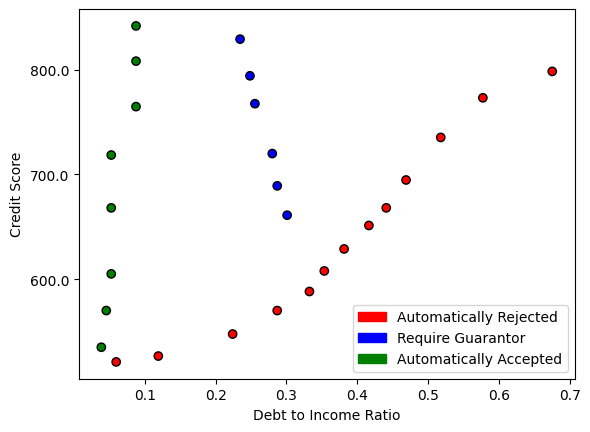
\includegraphics[width=.5\textwidth]{img_input/credit.png}
\end{center}
We've further transformed the raw data on debt to income ratio and credit score so that the default feature vector that you will be working with is defined as such:
\[\bm{x} = \left[\text{debt\_income\_ratio} \cdot \frac{200}{7}-7.5, \frac{\text{credit\_score}-500}{140}-0.5\right]^\top\]

\noindent Please implement the following classifiers in the \verb|SoftmaxRegression| and \verb|KNNClassifier| classes.


\begin{enumerate}[label=\alph*)]

  \item \textbf{A generative classifier with Gaussian class-conditional
          densities with a \textit{shared covariance} matrix} across all classes.
        Feel free to re-use your Problem 2 results.

  \item \textbf{Another generative classifier with Gaussian class-conditional densities , but now
          with a \textit{separate covariance} matrix} learned for each class. (Note:
        The staff implementation can switch between the two Gaussian generative classifiers with just a
        few lines of code.)

  \item \textbf{A multi-class logistic regression classifier} using the softmax activation function. In your implementation of gradient descent, \textbf{make sure to use L2 regularization} with regularization parameter $\lambda = 0.001$. Please also include a bias term, but do not regularize it. Limit the number of iterations of gradient descent to 200,000, and set the learning rate to be $\eta = 0.001$.

  \item \textbf{Another multi-class logistic regression classifier} with the additional feature map:
  $$\phi(\bm x) = [\ln (x_1+10), x_2^2]^\top$$

  \item \textbf{A kNN classifier} in which you classify based on the $k = 1$ and $k = 5$ nearest neighbors and the following distance function: 
  \[\text{dist}(\boldsymbol{x}, \boldsymbol{x}') = (x_1 - x'_1)^2/9 + (x_2 - x'_2)^2\]
        where nearest neighbors are those with the smallest distances from a given point.

        Note 1: When there are more than two labels, no label may have the
        majority of neighbors.  Use the label that has the most votes among
        the neighbors as the choice of label.

        Note 2: The grid of points for which you are making predictions
        should be interpreted as our test space.  Thus, it is not necessary
        to make a test point that happens to be on top of a training point
        ignore itself when selecting neighbors.

\end{enumerate}
\end{problem}

\newpage

\begin{framed}
  \noindent\textbf{Problem 3} (cont.)\\

After implementing the above classifiers, complete the following exercises:
  \begin{enumerate}



      \item Plot the decision boundaries generated by each classifier for the dataset. Include them in your PDF.
            Identify the similarities and differences among the classifiers. What explains the differences---in particular, which aspects or properties of each model dictate the shape of its decision boundary?
    
      \item
    
            Consider a loan applicant with Debt to Income Ratio 0.32 and Credit Score 350. To which class does each classifier assign this applicant? Report the classification probabilities of this applicant for models (c) and (d).
            
            Interpret how each model makes its classification decision. What else should we, the modelers, be aware of when making predictions on a point “far” from our training data? \textbf{Your response should no be longer than 5 sentences.}

    \item
        Can you think of any ethical problem that might arise from using this classifier to make loan decisions? You may approach this from any angle you like. For instance, can you think of someone who might have a low credit score and high debt-to-income ratio that you believe should nonetheless be offered a loan? Are there other variables that should be accounted for to ensure fair decisions? Are credit scores and debt-to-income ratio good bases for loan decisions? More generally, is using a classifier trained on past decisions to determine loan eligibility problematic in any way?
    \end{enumerate}
\end{framed}

\newpage

\begin{solution}

\begin{enumerate}
    \item[1.] The decision boundaries are plotted in Figures 3.1.1-6 below.
    \begin{figure}[H]
        \centering
        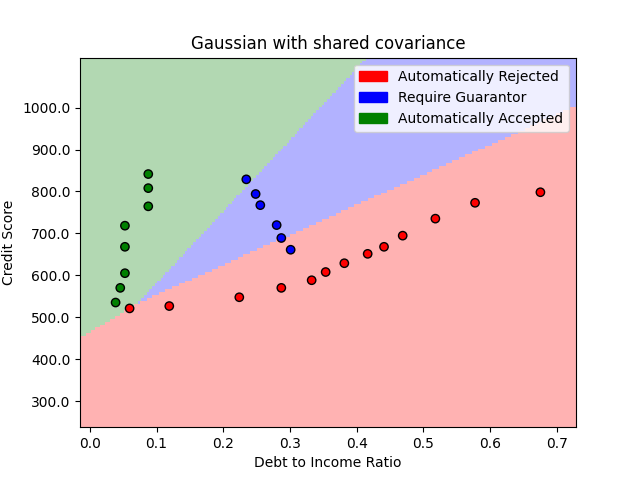
\includegraphics[width=0.6\textwidth]{img_output/Gaussian with shared covariance.png}
        \caption*{\textcolor{blue}{Figure 3.1.1: Gaussian with shared covariance matrix}}
        \label{fig:q3.1a}
    \end{figure}
    \begin{figure}[H]
        \centering
        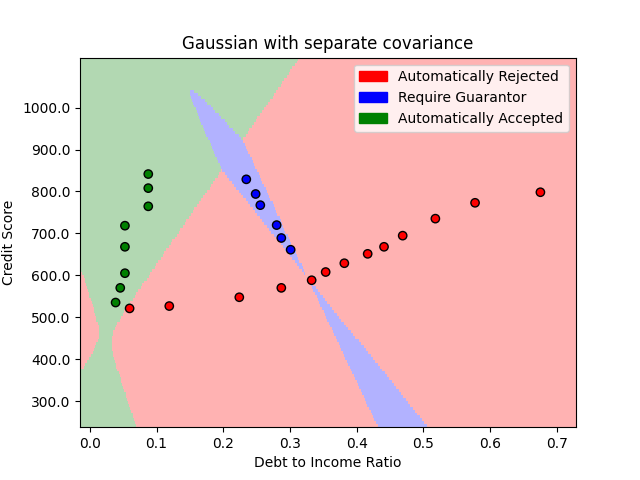
\includegraphics[width=0.65\textwidth]{img_output/Gaussian with separate covariance.png}
        \caption*{\textcolor{blue}{Figure 3.1.2: Gaussian with individual covariance matrices}}
        \label{fig:q3.1b}
    \end{figure}
    \begin{figure}[H]
        \centering
        \includegraphics[width=0.65\textwidth]{img_output/Softmax.png}
        \caption*{\textcolor{blue}{Figure 3.1.3: Softmax regression}}
        \label{fig:q3.1c}
    \end{figure}
    \begin{figure}[H]
        \centering
        \includegraphics[width=0.65\textwidth]{img_output/Softmax 2.png}
        \caption*{\textcolor{blue}{Figure 3.1.4: Softmax regression with additional feature map}}
        \label{fig:q3.1d}
    \end{figure}
    \begin{figure}[H]
        \centering
        \includegraphics[width=0.65\textwidth]{img_output/KNN, k=1.png}
        \caption*{\textcolor{blue}{Figure 3.1.5: kNN with k=1}}
        \label{fig:q3.1e}
    \end{figure}
    \begin{figure}[H]
        \centering
        \includegraphics[width=0.65\textwidth]{img_output/KNN, k=5.png}
        \caption*{\textcolor{blue}{Figure 3.1.6: kNN with k=5}}
        \label{fig:q3.1f}
    \end{figure}

    \clearpage
    Looking at the Gaussian generative classifiers in Figures 3.1.1\&2, we observe that the model with one shared covariance matrix has linear decision boundaries whereas the model with individual covariance matrices does not. Note that a decision boundary between two classes $k,l$ is defined by $p(\boldy_i = C_k | \boldx_i) = p(\boldy_i = C_l | \boldx_i)$. Recalling equation (2.3.1) we can see that when $\bSigma_k = \bSigma_l$, the quadratic terms in $\boldx_i$ cancel out, and so we are left with a linear equation (as observed in the boundaries in Figure 3.1.1). By contrast, when $\bSigma_k \neq \bSigma_l$, the quadratic term persists and we can get irregular boundaries. Note that using separate covariance allows for more nuanced classification.

    \vspace{.5em}
    Next, consider Figures 3.1.3\&4, which show the decision boundaries for the multi-class logistic regression models. Figure 3.1.3 shows linear decision boundaries. To understand why, note that the decision boundary is determined by the condition $p(\boldy_i = C_k | \boldx_i) = p(\boldy_i = C_l | \boldx_i)$. This is equivalent to $\text{softmax}(\mathbf{w}_k^\mathrm{T}\boldx_i) = \text{softmax}(\mathbf{w}_l^\mathrm{T}\boldx_i)$, which is equivalent to $(\mathbf{w}_k - \mathbf{w}_l)^\mathrm{T}\boldx_i = 0$, which is linear in $\boldx_i$. By contrast, in Figure 3.1.4, we first applied another basis transformation to the data $\boldx_i$. We can effectively think of $\boldx_{i2}^\prime = \sqrt{\ln (\boldx_{i1}^\prime + 10)}$ where $\boldx_i^\prime$ denotes the transformed data. This equation describes the shape of the curve seen in Figure 3.1.4.

    \vspace{.5em}
    Next, we look at Figures 3.1.5\&6. We observe that $k=1$ regions contain all the training points: This makes sense as if we have a new test point that is on top of the training point, it will use that training point as its prediction and be exactly correct. By contrast, for $k=5$, we can see that a couple of training points (red) are misclassified. Moreover, we can see that the lower part of the green (Class 2 = Automatically Accepted) boundary is shifted to the right for $k=5$. This reflects the fact that the majority of training points with $\boldx_{i1} < 0.1$ are green, and thus when a larger number of neighbors are considered, their influence outweighs that of the individual red points (versus the $k=1$ scenario). 

    \vspace{.5em}
    Finally, we make some general comparisons across the different regression methods. In particular, kNN has much more fragmented decision boundaries than do Gaussian or Softmax. This is because kNN is strongly influenced by local training points (which it takes the average of), whereas Gaussian and Softmax are parametric methods that assume a specific form for the decision boundary.

    \item[2.] The classifications are reported in Table 3.2.1 below:
\begin{table}[H]
    \centering
    \renewcommand{\arraystretch}{1.3} % Adjust row spacing
    \arrayrulecolor{blue} % Change border color to blue
    \begin{tabular}{|l|c|c|}
        \hline
        \textcolor{blue}{\textbf{Method}} & \textcolor{blue}{\textbf{Prediction}} & \textcolor{blue}{\textbf{Probabilities}} \\
        \hline
        \textcolor{blue}{Gaussian (shared cov matrix)} & \textcolor{blue}{0} & \textcolor{blue}{N/A} \\
        \hline
        \textcolor{blue}{Gaussian (separate cov matrix)} & \textcolor{blue}{0} & \textcolor{blue}{N/A} \\
        \hline
        \textcolor{blue}{Softmax} & \textcolor{blue}{0} & \textcolor{blue}{[1.0000e+00, 5.7319e-23, 1.5488e-33]} \\
        \hline
        \textcolor{blue}{Softmax (with extra feature map)} & \textcolor{blue}{1} & \textcolor{blue}{[2.1969e-01, 7.8024e-01, 7.2108e-05]} \\
        \hline
        \textcolor{blue}{kNN (k=1)} & \textcolor{blue}{0} & \textcolor{blue}{N/A} \\
        \hline
        \textcolor{blue}{kNN (k=5)} & \textcolor{blue}{0} & \textcolor{blue}{N/A} \\
        \hline
    \end{tabular}
    \caption*{\textcolor{blue}{Table 3.2.1: Prediction results for different models}}
\end{table}
    Suppose I have a new data point $\boldx_\text{new}$ and want to assign it a class $\boldy_\text{new} = C_l$, then we have the following interpretations for each model:
    \begin{enumerate}
        \item[1.] \textbf{Gaussian.} Assumes that the data within each class follow a Normal distribution and assigns $\boldx_\text{new}$ to the class with the highest (posterior) probability density, $p(\boldy_\text{new} = C_l | \boldx_\text{new})$. If $\boldx_\text{new}$ is ``far'' from our training data, caution is needed since it falls in the tail of the assumed normal distribution. If the real-world data deviates from a perfect Gaussian distribution, this could lead to significant errors in prediction.
        \item[2.] \textbf{Softmax.} Computes a score for each class, given by $\mathbf{w}^\mathrm{T}\boldx_\text{new}$. Assigns $\boldx_\text{new}$ to the class with the highest score. However, since Softmax \textit{normalizes} these scores (so as to assign a probability to each class), then it will always output a high probability for some class, even if $\boldx_\text{new}$ is very far from our train data. This is in contrast to the Gaussian model, where the probabilities themselves will be low to reflect the uncertainty.
        \item[3.] \textbf{kNN.} Assigns $\boldx_\text{new}$ to the majority class among its $k$-nearest neighbors. If $\boldx_\text{new}$ is very far from our train set, the $k$ neighbors will not be close at all, and thus our prediction may be very poor.
    \end{enumerate}

    \item[3.] There are several ethical concerns with using a classifier for such high-stakes decisions. First, credit score and debt-to-income ratio alone overlook important nuances among applicants. For instance, an applicant with a poor credit score and high debt-to-income ratio may not be financially irresponsible—if their payment history reveals they only spend on necessities, a human might approve the loan with a guarantor.

\vspace{.5em}
Second, many cases are borderline, and whilst a classifier may rigidly assign an applicant to one category over another based on a small probability difference, a human could weigh contextual factors and make a more flexible decision. That said, classifiers can serve as a valuable second opinion and work best alongside human oversight. A more robust model should incorporate situational factors (e.g., recent life events), spending patterns, credit mix, and alternative financial indicators (e.g., employment history, rent payments, etc.).

\vspace{.5em}
A final concern is that classifiers rely on past human decisions (the train data) to shape future ones. If historical decisions were biased (e.g., systematically denying certain groups), the classifier will reinforce and perpetuate that bias. Unlike humans, who may evolve in their decision-making, a classifier will continue to replicate historical patterns unless actively updated with new, bias-corrected data.
\end{enumerate}

\end{solution}

\clearpage
%%%%%%%%%%%%%%%%%%%%%%%%%%%%%%%%%%%%%%%%%%%%%
% Name and Calibration
%%%%%%%%%%%%%%%%%%%%%%%%%%%%%%%%%%%%%%%%%%%%%

\textbf{Name}: \textbf{\textcolor{blue}{Emma Harris}}

\vspace{.5em}
\textbf{Collaborators and Resources}: \textbf{\textcolor{blue}{N/A}}

\end{document}
